\section{Use cases}
To get an overview of the system functionality from a user's perspective, the team applied \glspl{usecase}, which is a technique to help developers identify what functionality that should be implemented, and possible errors that might occur in the system.

The primary actor in our system is the users of the Android application. A use case diagram of the final version of the system is shown in figure~\ref{fig:usecase}.

Functionality that was initially included in the requirement specification, but later left out, is discussed in chapter~\ref{sec:further}. 
For an overview of all textual use cases, see Appendix~\ref{sec:textUseCase}.\\

\begin{figure}[H]
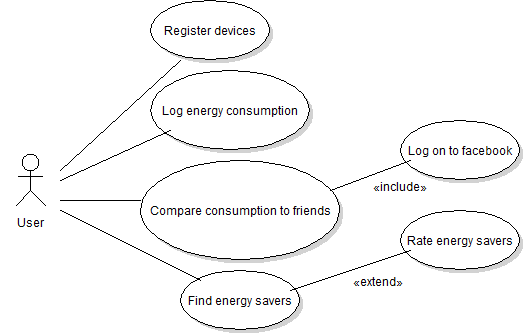
\includegraphics[width=\textwidth]{ch/specification/fig/currentUsecase.png}
\caption{Use case diagram for the entire system}
\label{fig:usecase}
\end{figure}
